% Options for packages loaded elsewhere
\PassOptionsToPackage{unicode}{hyperref}
\PassOptionsToPackage{hyphens}{url}
%
\documentclass[
  12pt,
]{article}
\usepackage{amsmath,amssymb}
\usepackage{iftex}
\ifPDFTeX
  \usepackage[T1]{fontenc}
  \usepackage[utf8]{inputenc}
  \usepackage{textcomp} % provide euro and other symbols
\else % if luatex or xetex
  \usepackage{unicode-math} % this also loads fontspec
  \defaultfontfeatures{Scale=MatchLowercase}
  \defaultfontfeatures[\rmfamily]{Ligatures=TeX,Scale=1}
\fi
\usepackage{lmodern}
\ifPDFTeX\else
  % xetex/luatex font selection
\fi
% Use upquote if available, for straight quotes in verbatim environments
\IfFileExists{upquote.sty}{\usepackage{upquote}}{}
\IfFileExists{microtype.sty}{% use microtype if available
  \usepackage[]{microtype}
  \UseMicrotypeSet[protrusion]{basicmath} % disable protrusion for tt fonts
}{}
\makeatletter
\@ifundefined{KOMAClassName}{% if non-KOMA class
  \IfFileExists{parskip.sty}{%
    \usepackage{parskip}
  }{% else
    \setlength{\parindent}{0pt}
    \setlength{\parskip}{6pt plus 2pt minus 1pt}}
}{% if KOMA class
  \KOMAoptions{parskip=half}}
\makeatother
\usepackage{xcolor}
\usepackage[margin=1in]{geometry}
\usepackage{color}
\usepackage{fancyvrb}
\newcommand{\VerbBar}{|}
\newcommand{\VERB}{\Verb[commandchars=\\\{\}]}
\DefineVerbatimEnvironment{Highlighting}{Verbatim}{commandchars=\\\{\}}
% Add ',fontsize=\small' for more characters per line
\usepackage{framed}
\definecolor{shadecolor}{RGB}{248,248,248}
\newenvironment{Shaded}{\begin{snugshade}}{\end{snugshade}}
\newcommand{\AlertTok}[1]{\textcolor[rgb]{0.94,0.16,0.16}{#1}}
\newcommand{\AnnotationTok}[1]{\textcolor[rgb]{0.56,0.35,0.01}{\textbf{\textit{#1}}}}
\newcommand{\AttributeTok}[1]{\textcolor[rgb]{0.13,0.29,0.53}{#1}}
\newcommand{\BaseNTok}[1]{\textcolor[rgb]{0.00,0.00,0.81}{#1}}
\newcommand{\BuiltInTok}[1]{#1}
\newcommand{\CharTok}[1]{\textcolor[rgb]{0.31,0.60,0.02}{#1}}
\newcommand{\CommentTok}[1]{\textcolor[rgb]{0.56,0.35,0.01}{\textit{#1}}}
\newcommand{\CommentVarTok}[1]{\textcolor[rgb]{0.56,0.35,0.01}{\textbf{\textit{#1}}}}
\newcommand{\ConstantTok}[1]{\textcolor[rgb]{0.56,0.35,0.01}{#1}}
\newcommand{\ControlFlowTok}[1]{\textcolor[rgb]{0.13,0.29,0.53}{\textbf{#1}}}
\newcommand{\DataTypeTok}[1]{\textcolor[rgb]{0.13,0.29,0.53}{#1}}
\newcommand{\DecValTok}[1]{\textcolor[rgb]{0.00,0.00,0.81}{#1}}
\newcommand{\DocumentationTok}[1]{\textcolor[rgb]{0.56,0.35,0.01}{\textbf{\textit{#1}}}}
\newcommand{\ErrorTok}[1]{\textcolor[rgb]{0.64,0.00,0.00}{\textbf{#1}}}
\newcommand{\ExtensionTok}[1]{#1}
\newcommand{\FloatTok}[1]{\textcolor[rgb]{0.00,0.00,0.81}{#1}}
\newcommand{\FunctionTok}[1]{\textcolor[rgb]{0.13,0.29,0.53}{\textbf{#1}}}
\newcommand{\ImportTok}[1]{#1}
\newcommand{\InformationTok}[1]{\textcolor[rgb]{0.56,0.35,0.01}{\textbf{\textit{#1}}}}
\newcommand{\KeywordTok}[1]{\textcolor[rgb]{0.13,0.29,0.53}{\textbf{#1}}}
\newcommand{\NormalTok}[1]{#1}
\newcommand{\OperatorTok}[1]{\textcolor[rgb]{0.81,0.36,0.00}{\textbf{#1}}}
\newcommand{\OtherTok}[1]{\textcolor[rgb]{0.56,0.35,0.01}{#1}}
\newcommand{\PreprocessorTok}[1]{\textcolor[rgb]{0.56,0.35,0.01}{\textit{#1}}}
\newcommand{\RegionMarkerTok}[1]{#1}
\newcommand{\SpecialCharTok}[1]{\textcolor[rgb]{0.81,0.36,0.00}{\textbf{#1}}}
\newcommand{\SpecialStringTok}[1]{\textcolor[rgb]{0.31,0.60,0.02}{#1}}
\newcommand{\StringTok}[1]{\textcolor[rgb]{0.31,0.60,0.02}{#1}}
\newcommand{\VariableTok}[1]{\textcolor[rgb]{0.00,0.00,0.00}{#1}}
\newcommand{\VerbatimStringTok}[1]{\textcolor[rgb]{0.31,0.60,0.02}{#1}}
\newcommand{\WarningTok}[1]{\textcolor[rgb]{0.56,0.35,0.01}{\textbf{\textit{#1}}}}
\usepackage{graphicx}
\makeatletter
\def\maxwidth{\ifdim\Gin@nat@width>\linewidth\linewidth\else\Gin@nat@width\fi}
\def\maxheight{\ifdim\Gin@nat@height>\textheight\textheight\else\Gin@nat@height\fi}
\makeatother
% Scale images if necessary, so that they will not overflow the page
% margins by default, and it is still possible to overwrite the defaults
% using explicit options in \includegraphics[width, height, ...]{}
\setkeys{Gin}{width=\maxwidth,height=\maxheight,keepaspectratio}
% Set default figure placement to htbp
\makeatletter
\def\fps@figure{htbp}
\makeatother
\setlength{\emergencystretch}{3em} % prevent overfull lines
\providecommand{\tightlist}{%
  \setlength{\itemsep}{0pt}\setlength{\parskip}{0pt}}
\setcounter{secnumdepth}{-\maxdimen} % remove section numbering
\usepackage{graphicx}
\usepackage{fancyhdr}
\usepackage{mdframed}
\pagestyle{fancy}
\fancyhead{}
\fancyhead[L]{\includegraphics[width=3cm]{logo.jpg}}
\fancyhead[R]{\hspace{0.5cm} Universidad Diego Portales \\ Facultad de Administración y Economía}
\fancypagestyle{plain}{ \fancyhead{} \fancyhead[L]{\includegraphics[width=3cm]{logo.jpg}} \fancyhead[R]{\hspace{0.5 cm} Universidad Diego Portales \\ Facultad de Administración y Economía}}
\usepackage{booktabs}
\usepackage{longtable}
\usepackage{array}
\usepackage{multirow}
\usepackage{wrapfig}
\usepackage{float}
\usepackage{colortbl}
\usepackage{pdflscape}
\usepackage{tabu}
\usepackage{threeparttable}
\usepackage{threeparttablex}
\usepackage[normalem]{ulem}
\usepackage{makecell}
\usepackage{xcolor}
\ifLuaTeX
  \usepackage{selnolig}  % disable illegal ligatures
\fi
\usepackage{bookmark}
\IfFileExists{xurl.sty}{\usepackage{xurl}}{} % add URL line breaks if available
\urlstyle{same}
\hypersetup{
  pdftitle={Ejercicio 5},
  hidelinks,
  pdfcreator={LaTeX via pandoc}}

\title{\textbf{Ejercicio 5}}
\author{}
\date{\vspace{-2.5em}}

\begin{document}
\maketitle

\maketitle
\vspace{-5em}
\vspace{0.5em}

\begin{center}
\footnotesize \textbf{Curso}: Econometría II \\
\footnotesize \textbf{Profesor}: Mauricio Tejada \\
\footnotesize \textbf{Estudiantes}: Dania Bustamante, Rosana Cardona, José Casanova \\
\footnotesize 26 junio 2024 \\
\end{center}

\subsection{\texorpdfstring{\textbf{\emph{Pregunta
1}}}{Pregunta 1}}\label{pregunta-1}

Calcule la tasa de crecimiento mensual de la variable INDPRO,
expresada\\
en términos porcentuales ¿Cuáles son la media y la desviación típica de
la variable gt durante el periodo muestral?

\begin{Shaded}
\begin{Highlighting}[]
\NormalTok{g\_t }\OtherTok{\textless{}{-}} \DecValTok{100} \SpecialCharTok{*} \FunctionTok{diff}\NormalTok{(}\FunctionTok{log}\NormalTok{(INDPRO))}

\NormalTok{media\_g\_t }\OtherTok{\textless{}{-}} \FunctionTok{mean}\NormalTok{(g\_t, }\AttributeTok{na.rm =} \ConstantTok{TRUE}\NormalTok{)}
\NormalTok{desviacion\_g\_t }\OtherTok{\textless{}{-}} \FunctionTok{sd}\NormalTok{(g\_t, }\AttributeTok{na.rm =} \ConstantTok{TRUE}\NormalTok{)}

\NormalTok{media\_g\_t}
\end{Highlighting}
\end{Shaded}

\begin{verbatim}
## [1] 0.2350164
\end{verbatim}

\begin{Shaded}
\begin{Highlighting}[]
\NormalTok{desviacion\_g\_t}
\end{Highlighting}
\end{Shaded}

\begin{verbatim}
## [1] 0.8828447
\end{verbatim}

La media de la tasa de crecimiento mensual es de 0.2350164.

La desviación tipica de la tasa de crecimiento mensual es de 0.8828447.

\subsection{\texorpdfstring{\textbf{\emph{Pregunta
2}}}{Pregunta 2}}\label{pregunta-2}

Represente gráficamente el valor de la variable Ot. ¿Por qué existen
tantos valores de Ot iguales a cero? ¿Por qué no existen valores de Ot
que sean negativos?

\includegraphics{Ejercicio-5_files/figure-latex/unnamed-chunk-2-1.pdf}

\begin{itemize}
\item
  \(O_t\) es igual a cero cuando el precio del petróleo en el periodo t
  no supera al máximo precio del año anterior. Esto sucede porque los
  precios del petróleo tienden a fluctuar y no siempre alcanzan un nuevo
  máximo cada mes.
\item
  La ausencia de valores negativos de \(O_t\) es la diferencia positiva
  entre el precio actual del petróleo y el máximo precio del año
  anterior. Si el precio del petróleo no supera al máximo del año
  anterior, es cero. Por lo tanto, no puede ser negativo.
\end{itemize}

\subsection{\texorpdfstring{\textbf{\emph{Pregunta
3}}}{Pregunta 3}}\label{pregunta-3}

Estime un modelo de Rezagos distribuidos para la variable gt sobre el
valor actual y los 18 valores retardados de la variable Ot. Estime los
errores estádnar HAC.

\subsubsection{\texorpdfstring{\textbf{\emph{Resumen del
modelo}}}{Resumen del modelo}}\label{resumen-del-modelo}

\begin{verbatim}
## 
## Time series regression with "ts" data:
## Start = 1959(7), End = 2013(12)
## 
## Call:
## dynlm(formula = formula, data = aligned_data)
## 
## Residuals:
##     Min      1Q  Median      3Q     Max 
## -3.8151 -0.4078  0.0097  0.3848  5.6295 
## 
## Coefficients:
##               Estimate Std. Error t value            Pr(>|t|)    
## (Intercept)  0.3683933  0.0366821  10.043 <0.0000000000000002 ***
## L(Ot, 0)     0.0067550  0.0129314   0.522              0.6016    
## L(Ot, 1)    -0.0201563  0.0137662  -1.464              0.1436    
## L(Ot, 2)    -0.0102141  0.0138368  -0.738              0.4607    
## L(Ot, 3)    -0.0061015  0.0138735  -0.440              0.6602    
## L(Ot, 4)    -0.0073852  0.0138773  -0.532              0.5948    
## L(Ot, 5)    -0.0103567  0.0138889  -0.746              0.4561    
## L(Ot, 6)    -0.0311658  0.0139014  -2.242              0.0253 *  
## L(Ot, 7)    -0.0009245  0.0138994  -0.067              0.9470    
## L(Ot, 8)     0.0058652  0.0138985   0.422              0.6732    
## L(Ot, 9)    -0.0187055  0.0139159  -1.344              0.1794    
## L(Ot, 10)   -0.0433425  0.0138985  -3.119              0.0019 ** 
## L(Ot, 11)   -0.0351425  0.0138994  -2.528              0.0117 *  
## L(Ot, 12)   -0.0005823  0.0139014  -0.042              0.9666    
## L(Ot, 13)   -0.0150695  0.0138889  -1.085              0.2783    
## L(Ot, 14)   -0.0119535  0.0138773  -0.861              0.3894    
## L(Ot, 15)   -0.0165019  0.0138735  -1.189              0.2347    
## L(Ot, 16)   -0.0036165  0.0138368  -0.261              0.7939    
## L(Ot, 17)    0.0098934  0.0137662   0.719              0.4726    
## L(Ot, 18)    0.0087075  0.0129314   0.673              0.5010    
## ---
## Signif. codes:  0 '***' 0.001 '**' 0.01 '*' 0.05 '.' 0.1 ' ' 1
## 
## Residual standard error: 0.7778 on 634 degrees of freedom
##   (35 observations deleted due to missingness)
## Multiple R-squared:  0.1212, Adjusted R-squared:  0.0949 
## F-statistic: 4.604 on 19 and 634 DF,  p-value: 0.0000000005574
\end{verbatim}

\subsubsection{\texorpdfstring{\textbf{\emph{Errores Estandar
HAC}}}{Errores Estandar HAC}}\label{errores-estandar-hac}

\begin{verbatim}
## 
## t test of coefficients:
## 
##                Estimate  Std. Error t value            Pr(>|t|)    
## (Intercept)  0.36839325  0.04710952  7.8199 0.00000000000002213 ***
## L(Ot, 0)     0.00675505  0.00918379  0.7355             0.46228    
## L(Ot, 1)    -0.02015629  0.00799159 -2.5222             0.01191 *  
## L(Ot, 2)    -0.01021408  0.00926500 -1.1024             0.27069    
## L(Ot, 3)    -0.00610150  0.00938333 -0.6502             0.51577    
## L(Ot, 4)    -0.00738521  0.00994010 -0.7430             0.45777    
## L(Ot, 5)    -0.01035674  0.00701386 -1.4766             0.14028    
## L(Ot, 6)    -0.03116576  0.01700201 -1.8331             0.06726 .  
## L(Ot, 7)    -0.00092449  0.01100854 -0.0840             0.93310    
## L(Ot, 8)     0.00586515  0.01259454  0.4657             0.64160    
## L(Ot, 9)    -0.01870549  0.01174127 -1.5931             0.11163    
## L(Ot, 10)   -0.04334246  0.02448840 -1.7699             0.07722 .  
## L(Ot, 11)   -0.03514250  0.02265619 -1.5511             0.12137    
## L(Ot, 12)   -0.00058233  0.01503298 -0.0387             0.96911    
## L(Ot, 13)   -0.01506948  0.01338388 -1.1259             0.26062    
## L(Ot, 14)   -0.01195346  0.01098888 -1.0878             0.27711    
## L(Ot, 15)   -0.01650189  0.00914252 -1.8050             0.07156 .  
## L(Ot, 16)   -0.00361647  0.00902037 -0.4009             0.68861    
## L(Ot, 17)    0.00989343  0.00813700  1.2159             0.22449    
## L(Ot, 18)    0.00870750  0.01051423  0.8282             0.40789    
## ---
## Signif. codes:  0 '***' 0.001 '**' 0.01 '*' 0.05 '.' 0.1 ' ' 1
\end{verbatim}

\subsection{\texorpdfstring{\textbf{\emph{Pregunta
4}}}{Pregunta 4}}\label{pregunta-4}

Considerados de forma conjunta, ¿son los coeficientes de Ot estadística
y significativamente distintos de cero?

\[H_o: Todos\ los\ rezagos\ son\ cero \]
\[H_1: Al\ menos\ uno\ es\ diferente\ cero \]

\begin{verbatim}
## Linear hypothesis test
## 
## Hypothesis:
## L(Ot, 0) = 0
## L(Ot,0
## L(Ot, 2) = 0
## L(Ot, 3) = 0
## L(Ot, 4) = 0
## L(Ot, 5) = 0
## L(Ot, 6) = 0
## L(Ot, 7) = 0
## L(Ot, 8) = 0
## L(Ot, 9) = 0
## L(Ot, 10) = 0
## L(Ot, 11) = 0
## L(Ot, 12) = 0
## L(Ot, 13) = 0
## L(Ot, 14) = 0
## L(Ot, 15) = 0
## L(Ot, 16) = 0
## L(Ot, 17) = 0
## L(Ot, 18) = 0
## 
## Model 1: restricted model
## Model 2: g_t ~ L(Ot, 0) + L(Ot, 1) + L(Ot, 2) + L(Ot, 3) + L(Ot, 4) + 
##     L(Ot, 5) + L(Ot, 6) + L(Ot, 7) + L(Ot, 8) + L(Ot, 9) + L(Ot, 
##     10) + L(Ot, 11) + L(Ot, 12) + L(Ot, 13) + L(Ot, 14) + L(Ot, 
##     15) + L(Ot, 16) + L(Ot, 17) + L(Ot, 18)
## 
##   Res.Df    RSS Df Sum of Sq      F          Pr(>F)    
## 1    653 436.48                                        
## 2    634 383.56 19    52.918 4.6036 0.0000000005574 ***
## ---
## Signif. codes:  0 '***' 0.001 '**' 0.01 '*' 0.05 '.' 0.1 ' ' 1
\end{verbatim}

Si el valor p es menor que el nivel de significancia \(\alpha=0,5\),
rechazamos la hipótesis nula de que todos los coeficientes de los
rezagos son cero. Esto nos dice que al menos uno de los coeficientes es
estadísticamente significativo.

\textbf{\emph{Resultados}}

Modelo restringido (sin Rezagos):

\begin{itemize}
\tightlist
\item
  gl: 653
\item
  SRC: 436.48
\end{itemize}

Modelo completo (con Rezagos):

\begin{itemize}
\tightlist
\item
  gl: 634
\item
  SRC: 383.56
\end{itemize}

Diferencia en sumas de cuadrados: 52.918

Estadístico F: 4.6036

Valor p: 0.0000000005574 (menor que 0.05)

\begin{itemize}
\tightlist
\item
  Dado que el valor p es menor al nivel de significancia, rechazamos la
  hipótesis nula de que todos los coeficientes de los rezagos son cero.
  Esto nos dice que los rezagos tienen un efecto estadísticamente
  significativo sobre la variable dependiente en conjunto, sugiriendo
  que tienen un impacto en la variable de interés.
\end{itemize}

\subsection{\texorpdfstring{\textbf{\emph{Pregunta
5}}}{Pregunta 5}}\label{pregunta-5}

Realice unos gráficos como los vistos en clase representando los
multiplicadores dinámicos estimados, los multiplicadores acumulativos, y
los intervalos de confianza al 95\%. Comente su opinión acerca del
tamaño de los multiplicadores en la realidad.

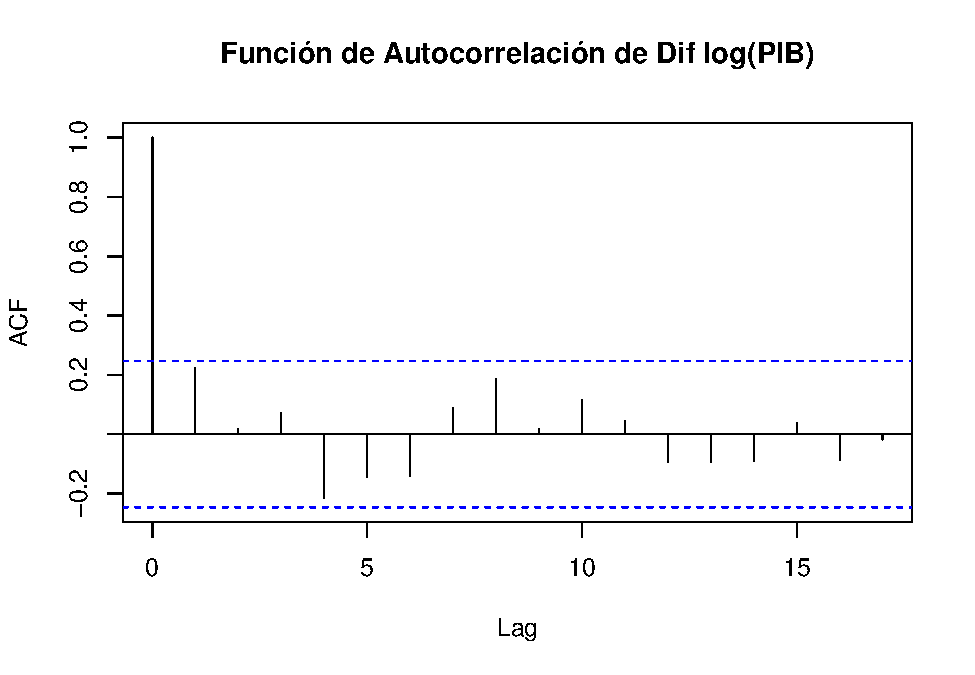
\includegraphics{Ejercicio-5_files/figure-latex/unnamed-chunk-8-1.pdf}

Los multiplicadores dinámicos muestran que los efectos directos de
\(Ot\) sobre \(gt\) son variables y en su mayoría no significativos.
Esto podría indicar que los cambios en los precios del petróleo no
tienen un impacto fuerte y consistente en la producción industrial en
cada periodo individual.

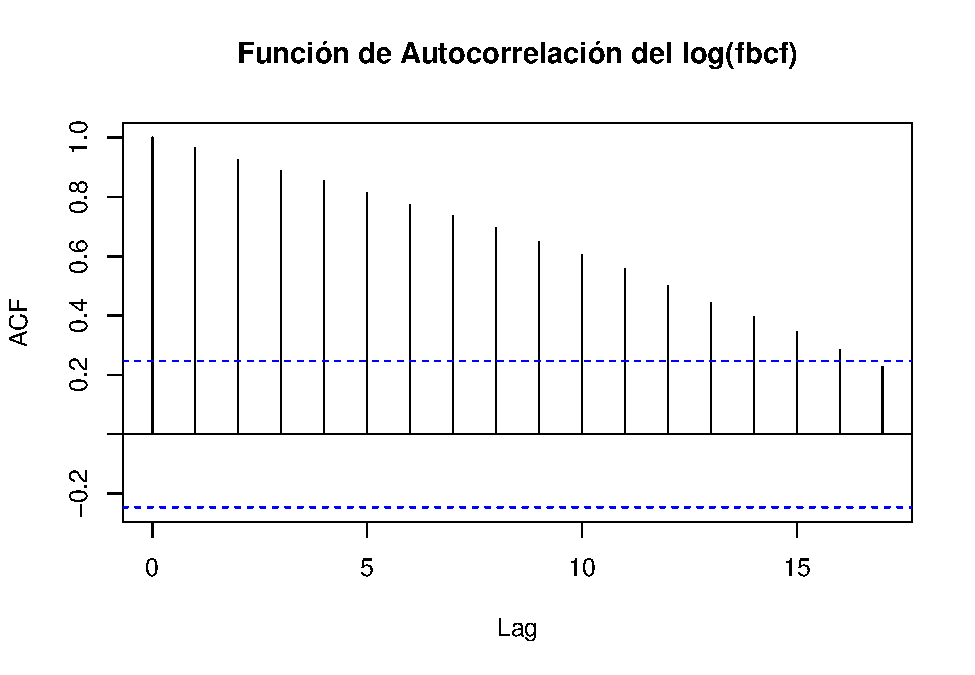
\includegraphics{Ejercicio-5_files/figure-latex/unnamed-chunk-9-1.pdf}

Los multiplicadores acumulativos muestran un impacto negativo
acumulativo a lo largo del tiempo, aunque con alta incertidumbre. Esto
podría interpretarse como que, aunque los efectos individuales no son
significativos, hay una tendencia general de que los aumentos en los
precios del petróleo tienden a reducir la producción en el largo plazo.
Sin embargo, la alta incertidumbre que muestra los intervalos de
confianza amplios indica que estas conclusiones pueden ser erroneas.

\textbf{\emph{Resumiendo:}}

\begin{enumerate}
\def\labelenumi{\arabic{enumi}.}
\item
  La mayoría de los efectos dinámicos no son estadísticamente
  significativos, y existe una alta incertidumbre en los efectos
  acumulativos.
\item
  A pesar de la falta de significancia estadística en muchos puntos, se
  encuentra que existe un posible impacto acumulativo negativo de los
  aumentos en los precios del petróleo sobre la producción.
\item
  Debido a la alta incertidumbre, la conclusión sobre el impacto de los
  precios del petróleo debe tomarse con cuidado y tomar en cuenta con
  otros factores económicos. \newpage
\end{enumerate}

\subsection{\texorpdfstring{\textbf{\emph{Pregunta
6}}}{Pregunta 6}}\label{pregunta-6}

Supóngase que la elevada demanda de Estados Unidos (evidenciada por los
elevados valores de la variable gt) conduce a un aumento en los precios
del petróleo. ¿Es exógena la variable Ot? Resultan confiables los
multiplicadores estimados que se muestran en los gráficos anteriores?
Explíquelo.

\textbf{\emph{Exogeneidad de}} \(Ot\)\textbf{\emph{:}}

\begin{itemize}
\item
  Si se considera que la elevada demanda de Estados Unidos genera un
  aumento en los precios del petróleo, esto indica que la varible \(Ot\)
  no es exógena, lo cual viola el supuesto de exogeneidad.
\item
  Si \(Ot\) no es exogena esto implica que los errores del modelo pueden
  estar correlacionados , generando un sesgo en las estimaciones de los
  coeficientes.
\item
  Los multiplicadores asumen que \(Ot\) es exógena. Si no es exógena,
  los multiplicadores no reflejan de manera correcta el efecto causal
  entre \(Ot\) y \(gt\) .
\item
  La presencia de endogeneidad genera sesgo en las estimaciones,
  afectando la confiabilidad de los multiplicadores de los gráficos
  anteriores.
\item
  Los intervalos de confianza también pueden ser incorrectos si \(Ot\)
  no es exógena, ya que no muestran de manera adecuada la incertidumbre
  en las estimaciones.
\end{itemize}

\end{document}
